\section{自然梯度}
\label{sec:igeo-natural-gradient}

第~\ref{chap:distribution-approximation}章在参数族$\{Q_{\bm{\theta}}\}$中逼近目标分布$\Pi$，目标函数$L(\bm{\theta})$例如取$D_{\mathrm{KL}}(Q_{\bm{\theta}}\Vert\Pi)$或$D_{\mathrm{KL}}(\Pi\Vert Q_{\bm{\theta}})$。这样的目标是参数的可微函数时，最直接的更新是沿负梯度走一步：$\bm{\theta}\leftarrow\bm{\theta}-\alpha\nabla_{\bm{\theta}}L$。上一节已经看到，参数的同一段欧氏长度在不同位置、不同坐标下代表的分布变化相差悬殊，按欧氏长度分配步伐并没有道理。更合理的问法是：在允许分布发生同样大小的局部变化时，哪个方向使目标下降最多？

本节用一个能手算的例子贯穿。目标分布取$\Pi=\mathcal{N}(0,1)$，候选族为$Q_{\mu,v}=\mathcal{N}(\mu,v)$，目标函数取第~\ref{chap:distribution-approximation}章的$D_{\mathrm{KL}}(Q\Vert\Pi)$。由第~\ref{chap:distribution-comparison}章的高斯KL公式，
\begin{equation}
  L(\mu,v)=-\frac12\ln v+\frac{v+\mu^{2}}{2}-\frac12 .
  \label{eq:igeo-running-objective}
\end{equation}
为了每一步都能核对，这里的目标就在候选族内，最优解$(\mu,v)=(0,1)$是已知的。起点取$\mathcal{N}(1,4)$，那里$L=-\ln2+2\approx1.3069$。

\subsection{受限的下降方向}
\label{sec:igeo-steepest}

记$\bm{g}=\nabla_{\bm{\theta}}L(\bm{\theta})$。参数走一小步$\bm{\delta}$，目标的一阶变化是$\langle\bm{g},\bm{\delta}\rangle$；由定理~\ref{thm:igeo-kl-expansion}，分布的局部变化约为Fisher二次型的一半。给定一个KL预算$\varepsilon>0$，考虑问题
\begin{equation}
  \min_{\bm{\delta}\in\mathbb{R}^{k}}\ \langle\bm{g},\bm{\delta}\rangle\qquad\text{s.t.}\qquad\frac12\bm{\delta}^{\top}\bm{G}(\bm{\theta})\bm{\delta}\leq\varepsilon .
  \label{eq:igeo-steepest-problem}
\end{equation}
若把约束换成$\lVert\bm{\delta}\rVert_2\leq r$，答案是$-\bm{g}$的方向，这就是普通梯度下降。约束换成Fisher二次型以后，答案改变。

\begin{theorem}[Fisher度量下的最速下降方向]
\label{thm:igeo-steepest}
设$\bm{G}=\bm{G}(\bm{\theta})$正定，$\bm{g}\neq\bm{0}$。则问题~\eqref{eq:igeo-steepest-problem}有唯一解
\begin{equation}
  \bm{\delta}^{*}=-\sqrt{\frac{2\varepsilon}{\bm{g}^{\top}\bm{G}^{-1}\bm{g}}}\;\bm{G}^{-1}\bm{g},
  \label{eq:igeo-steepest-solution}
\end{equation}
最小值为
\begin{equation}
  \langle\bm{g},\bm{\delta}^{*}\rangle=-\sqrt{2\varepsilon\,\bm{g}^{\top}\bm{G}^{-1}\bm{g}} .
  \label{eq:igeo-steepest-value}
\end{equation}
\end{theorem}

\begin{proof}
$\bm{G}$正定，所以
\[
  \langle\bm{a},\bm{b}\rangle_{\bm{G}}=\bm{a}^{\top}\bm{G}\bm{b}
\]
是$\mathbb{R}^{k}$上的内积，记相应的范数为$\lVert\cdot\rVert_{\bm{G}}$，约束就是$\bm{\delta}$的这个范数不超过$\sqrt{2\varepsilon}$。把目标的一阶变化写成这个内积：
\[
  \langle\bm{g},\bm{\delta}\rangle=(\bm{G}^{-1}\bm{g})^{\top}\bm{G}\bm{\delta}=\langle\bm{G}^{-1}\bm{g},\bm{\delta}\rangle_{\bm{G}} .
\]
由Cauchy--Schwarz不等式与约束，
\[
  \langle\bm{G}^{-1}\bm{g},\bm{\delta}\rangle_{\bm{G}}\geq-\lVert\bm{G}^{-1}\bm{g}\rVert_{\bm{G}}\,\lVert\bm{\delta}\rVert_{\bm{G}}\geq-\sqrt{\bm{g}^{\top}\bm{G}^{-1}\bm{g}}\,\sqrt{2\varepsilon},
\]
这里用了
\[
  \lVert\bm{G}^{-1}\bm{g}\rVert_{\bm{G}}^{2}=\bm{g}^{\top}\bm{G}^{-1}\bm{G}\bm{G}^{-1}\bm{g}=\bm{g}^{\top}\bm{G}^{-1}\bm{g}.
\]
第一个不等号取等当且仅当$\bm{\delta}=-c\,\bm{G}^{-1}\bm{g}$，$c\geq0$；第二个取等当且仅当$\bm{\delta}$落在椭圆的边界上。两者同时成立唯一确定$c$，即式~\eqref{eq:igeo-steepest-solution}；代入目标，得到式~\eqref{eq:igeo-steepest-value}。
\end{proof}

最优方向与预算$\varepsilon$无关，$\varepsilon$只决定走多远。这个方向值得单独命名。

\begin{definition}[自然梯度]
\label{def:igeo-natural-gradient}
设$\bm{G}(\bm{\theta})$正定。称
\begin{equation}
  \widetilde{\nabla}L(\bm{\theta})=\bm{G}(\bm{\theta})^{-1}\nabla_{\bm{\theta}}L(\bm{\theta})
  \label{eq:igeo-natural-gradient}
\end{equation}
为$L$在$\bm{\theta}$处的\term{自然梯度}（natural gradient）。
\end{definition}

普通梯度相当于假定参数空间各处、各方向的尺度都一样，相当于在一张比例尺处处相同的地图上找最陡的方向。Fisher信息说明这张地图的比例尺因地因向而异：$\bm{G}$大的方向，参数稍动分布就大变，走一小步就要花掉很多预算；$\bm{G}$小的方向，参数要走很远分布才有同样的变化。自然梯度用$\bm{G}^{-1}$把梯度重新分配到这些方向上，便宜的方向多走，贵的方向少走。类比的边界在于，Fisher尺度只在局部成立，它不告诉我们走远以后路面怎样。

\paragraph{例中的两个方向}
在$(\mu,v)$坐标下，由式~\eqref{eq:igeo-running-objective}，
\[
  \bm{g}=\Bigl(\mu,\ \frac12-\frac{1}{2v}\Bigr),\qquad\bm{G}=\begin{bmatrix}1/v&0\\0&1/(2v^{2})\end{bmatrix}.
\]
在起点$(1,4)$处，
\[
  \bm{g}=(1,\ 0.375),\qquad\bm{G}=\operatorname{diag}\bigl(\tfrac14,\ \tfrac1{32}\bigr),\qquad\bm{G}^{-1}\bm{g}=(4,\ 12),
\]
并且$\bm{g}^{\top}\bm{G}^{-1}\bm{g}=4+4.5=8.5$。普通梯度主要指向$\mu$，自然梯度却主要指向$v$：在$v=4$处，$G_{vv}=\frac1{32}$很小，改变方差很“便宜”。

取预算$\varepsilon=0.05$。由式~\eqref{eq:igeo-steepest-solution}，自然梯度步为
\[
  \bm{\delta}_{\mathrm{nat}}=-\sqrt{\frac{0.1}{8.5}}\,(4,\ 12)\approx(-0.434,\ -1.302),
\]
目标的一阶下降为$\sqrt{2\varepsilon\cdot8.5}\approx0.922$。把$-\bm{g}$缩放成$-t\bm{g}$并放到同一个椭圆上，需要
\[
  \frac12t^{2}\,\bm{g}^{\top}\bm{G}\bm{g}=\varepsilon ,
\]
而$\bm{g}^{\top}\bm{G}\bm{g}\approx0.2544$，于是$t\approx0.627$，
\[
  \bm{\delta}_{\mathrm{euc}}=-0.627\,(1,\ 0.375)\approx(-0.627,\ -0.235),
\]
一阶下降为$0.627\times1.1406\approx0.715$。实际代入式~\eqref{eq:igeo-running-objective}，两步之后的目标值分别是$0.513$与$0.789$，起点为$1.307$。

\begin{BookInlineFigure}
  \centering
  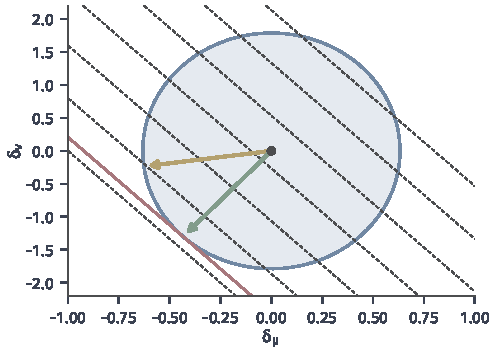
\includegraphics[width=84mm]{figures/07-probability/07-distribution-optimization/matplotlib/igeo-steepest-descent/figure.pdf}
  \caption{$\mathcal{N}(1,4)$处问题~\eqref{eq:igeo-steepest-problem}的几何，坐标为位移$(\delta_{\mu},\delta_{v})$。蓝色椭圆为$\frac12\bm{\delta}^{\top}\bm{G}\bm{\delta}=0.05$，深灰虚线为一阶变化$\langle\bm{g},\bm{\delta}\rangle$的等值线，红线是与椭圆相切的最低等值线。绿色箭头为自然梯度步，黄色箭头为缩放到同一椭圆上的负梯度。}
  \label{fig:igeo-steepest-descent}
\end{BookInlineFigure}

图~\ref{fig:igeo-steepest-descent}把问题~\eqref{eq:igeo-steepest-problem}画了出来。目标的一阶变化在位移平面上是一族平行直线，可行集是Fisher椭圆。最优点是椭圆与最低一条等值线的切点，它在绿色箭头的末端；黄色箭头末端所在的等值线高出不少。这里两个方向的一阶下降比约为$0.78$，差距来自椭圆的扁平程度：在$\bm{G}$各向同性的点，两个方向重合。

把预算想成固定大小的步伐，问题~\eqref{eq:igeo-steepest-problem}就是一种信赖域子问题：在可信的范围内用线性模型选方向，只是范围由分布的变化而不是参数的欧氏距离来划定，可参考\BookChapterRef{chap:trust-region}{卷五第9章“信赖域”}。若$\Pi$本身在候选族内，在最优点$\bm{\theta}^{*}$附近，$D_{\mathrm{KL}}(Q_{\bm{\theta}}\Vert\Pi)$恰好就是$Q_{\bm{\theta}}$与$Q_{\bm{\theta}^{*}}$之间的KL散度，它的Hessian在$\bm{\theta}^{*}$处等于$\bm{G}(\bm{\theta}^{*})$；这时自然梯度在最优点附近与Newton方向几乎一致。

\paragraph{信息矩阵退化时}
定理~\ref{thm:igeo-steepest}要求$\bm{G}$正定。$\bm{G}$奇异时，不能直接写$\bm{G}^{-1}$，而要先回到第~\ref{sec:igeo-fisher}节，辨认退化来自参数冗余还是一阶失效，在有效的坐标上重新建立问题。

先看参数冗余。在$\mathcal{N}(a+b,1)$中逼近$\Pi=\mathcal{N}(1,1)$，记$c=a+b$，目标是$L=\frac12(c-1)^{2}$。梯度与信息矩阵分别是
\[
  \bm{g}=(c-1)\begin{bmatrix}1\\1\end{bmatrix},\qquad\bm{G}=\begin{bmatrix}1&1\\1&1\end{bmatrix}.
\]
$\bm{G}$的零空间沿$(1,-1)$，沿这个方向分布不变，目标也不变，所以$\bm{g}$自动与它正交。去掉冗余，直接用$c$作参数，$G_{cc}=1$，自然梯度是$c-1$。若坚持在$(a,b)$中计算，可以用Moore--Penrose伪逆，$\bm{G}^{\dagger}\bm{g}=\frac{c-1}{2}(1,1)$，它在$c$上引起的变化同样是$c-1$；伪逆只是从无穷多个等价的位移中选了欧氏长度最短的那一个，零空间方向上走多少是任意约定。

再看一阶失效。在$\mathcal{N}(\theta^{3},1)$中逼近同一个$\Pi$，目标是$L=\frac12(\theta^{3}-1)^{2}$，
\[
  g(\theta)=3\theta^{2}(\theta^{3}-1),\qquad G(\theta)=9\theta^{4},\qquad\frac{g(\theta)}{G(\theta)}=\frac{\theta^{3}-1}{3\theta^{2}} .
\]
在$\theta=0$处普通梯度为零，$\theta=0$是$L$的驻点，可分布$\mathcal{N}(0,1)$离最优的$\mathcal{N}(1,1)$还很远；自然梯度则在$\theta\to0$时趋于无穷。两者都是坐标的毛病：用均值$m=\theta^{3}$作参数，$G_{mm}=1$，自然梯度是$m-1$，在$m=0$附近完全正常。

\begin{BookInlineFigure}
  \centering
  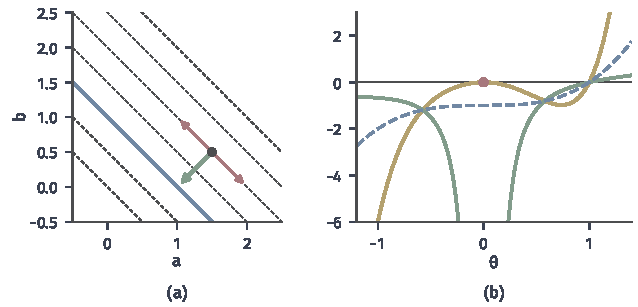
\includegraphics[width=108mm]{figures/07-probability/07-distribution-optimization/matplotlib/igeo-degenerate/figure.pdf}
  \caption{信息矩阵退化的两种情形。(a)$\mathcal{N}(a+b,1)$逼近$\mathcal{N}(1,1)$：深灰虚线是$a+b$为常数的直线，其上分布相同，蓝线$a+b=1$是全部最优参数；在$(1.5,0.5)$处，红色双箭头为$\bm{G}$的零空间方向，绿色箭头为伪逆给出的下降位移。(b)$\mathcal{N}(\theta^{3},1)$逼近$\mathcal{N}(1,1)$：黄线为普通梯度$3\theta^{2}(\theta^{3}-1)$，在红点$\theta=0$处为零；绿线为$g/G=(\theta^{3}-1)/(3\theta^{2})$，在$0$附近发散；蓝色虚线为均值坐标下的自然梯度$m-1$，按$m=\theta^{3}$画在$\theta$轴上。}
  \label{fig:igeo-degenerate}
\end{BookInlineFigure}

图~\ref{fig:igeo-degenerate}对照了这两种情形。实践中常用的另一个办法是把$\bm{G}$换成$\bm{G}+\gamma\bm{I}$，$\gamma>0$，矩阵总是可逆。它能防止数值上的崩溃，却没有回答问题：(b)中$\theta$接近$0$时，加上$\gamma$以后的方向主要由$\gamma$的大小决定，而不是由分布的变化决定。先识别退化方向，再在有效坐标上建立问题，加正则项只作为数值上的保护。

\subsection{重参数化后的更新}
\label{sec:igeo-reparam-update}

普通梯度依赖坐标，这一点从变换公式就能看出。设$\bm{\theta}=\bm{\varphi}(\bm{\xi})$，Jacobian为$\bm{J}$，由链式法则，同一个目标函数在两套坐标中的梯度满足
\[
  \bm{g}_{\bm{\xi}}=\bm{J}^{\top}\bm{g}_{\bm{\theta}} .
\]
在$\bm{\xi}$坐标中沿$-\bm{g}_{\bm{\xi}}$走一小步，换算到$\bm{\theta}$坐标，位移是
\[
  -\bm{J}\bm{g}_{\bm{\xi}}=-\bm{J}\bm{J}^{\top}\bm{g}_{\bm{\theta}} .
\]
除非$\bm{J}\bm{J}^{\top}=\bm{I}$，它与在$\bm{\theta}$坐标中沿$-\bm{g}_{\bm{\theta}}$走的位移不同：两种坐标下的“梯度下降”是两个不同的方向。

自然梯度没有这个问题。由式~\eqref{eq:igeo-reparam}，$\bm{G}^{\Xi}=\bm{J}^{\top}\bm{G}\bm{J}$，于是
\begin{equation}
  \bm{J}\,(\bm{G}^{\Xi})^{-1}\bm{g}_{\bm{\xi}}=\bm{J}\,\bm{J}^{-1}\bm{G}^{-1}\bm{J}^{-\top}\bm{J}^{\top}\bm{g}_{\bm{\theta}}=\bm{G}^{-1}\bm{g}_{\bm{\theta}} .
  \label{eq:igeo-natural-invariance}
\end{equation}
$\bm{\xi}$坐标中的自然梯度换算到$\bm{\theta}$坐标，恰好是$\bm{\theta}$坐标中的自然梯度，两者是同一个切向量。同样，
\[
  \bm{g}_{\bm{\xi}}^{\top}(\bm{G}^{\Xi})^{-1}\bm{g}_{\bm{\xi}}=\bm{g}_{\bm{\theta}}^{\top}\bm{G}^{-1}\bm{g}_{\bm{\theta}},
\]
自然梯度在Fisher度量下的长度也与坐标无关。这与定理~\ref{thm:igeo-steepest}一致：问题~\eqref{eq:igeo-steepest-problem}的目标与约束都只依赖分布，答案自然不依赖于怎样给分布编号。

\paragraph{例中的核对}
把例子改写到自然参数。两套坐标之间的变换是
\[
  (\theta_1,\theta_2)=\Bigl(\frac{\mu}{v},\,-\frac{1}{2v}\Bigr),\qquad(\mu,v)=\Bigl(-\frac{\theta_1}{2\theta_2},\,-\frac{1}{2\theta_2}\Bigr),
\]
起点$\mathcal{N}(1,4)$对应$\bm{\theta}=(0.25,\,-0.125)$。后一个变换的Jacobian在起点处为
\[
  \bm{J}=\frac{\partial(\mu,v)}{\partial(\theta_1,\theta_2)}=\begin{bmatrix}-\frac{1}{2\theta_2}&\frac{\theta_1}{2\theta_2^{2}}\\0&\frac{1}{2\theta_2^{2}}\end{bmatrix}=\begin{bmatrix}4&8\\0&32\end{bmatrix}.
\]
这里$\bm{\theta}$扮演新坐标$\bm{\xi}$的角色。由$\bm{g}_{\bm{\theta}}=\bm{J}^{\top}\bm{g}_{\mu,v}$，
\[
  \bm{g}_{\bm{\theta}}=\begin{bmatrix}4&0\\8&32\end{bmatrix}\begin{bmatrix}1\\0.375\end{bmatrix}=\begin{bmatrix}4\\20\end{bmatrix}.
\]

由式~\eqref{eq:igeo-reparam}算出的信息矩阵是
\[
  \bm{J}^{\top}\begin{bmatrix}\frac14&0\\0&\frac1{32}\end{bmatrix}\bm{J}=\begin{bmatrix}4&8\\8&48\end{bmatrix},
\]
正是第~\ref{sec:igeo-exponential}节由式~\eqref{eq:igeo-gauss-natural-fisher}得到的矩阵。解$\bm{G}\bm{d}=\bm{g}_{\bm{\theta}}$得$\bm{d}=(0.25,\,0.375)$，换算回去，
\[
  \bm{J}\bm{d}=\begin{bmatrix}4\cdot0.25+8\cdot0.375\\32\cdot0.375\end{bmatrix}=\begin{bmatrix}4\\12\end{bmatrix},
\]
正是$(\mu,v)$坐标中的自然梯度，并且$\bm{g}_{\bm{\theta}}^{\top}\bm{d}=1+7.5=8.5$与前面相同。

普通梯度则不然：自然参数中的负梯度$-(4,20)$换算到$(\mu,v)$坐标，是
\[
  -\bm{J}\begin{bmatrix}4\\20\end{bmatrix}=-\begin{bmatrix}176\\640\end{bmatrix},
\]
与$(\mu,v)$坐标中的负梯度$-(1,\ 0.375)$方向不同。

\paragraph{有限步的差别}
自然梯度给出的是切方向，实际更新还要走一个有限步。最简单的规则是在当前坐标中直接相加：$\bm{\theta}\leftarrow\bm{\theta}-\alpha\,\bm{G}^{-1}\bm{g}$。三套坐标下的方向在起点相切，但各自是“直线”的那条曲线并不相同，走出有限距离后到达的分布也不同。

取$\alpha=\frac18$，从$\mathcal{N}(1,4)$出发，在三套坐标中各走一步。在$(\mu,v)$坐标中，自然梯度为$(4,12)$，
\[
  (\mu,v)\leftarrow(1-\tfrac12,\ 4-\tfrac32)=(0.5,\ 2.5).
\]
在自然参数中，自然梯度为$(0.25,0.375)$，
\[
  \bm{\theta}\leftarrow(0.25,\,-0.125)-\tfrac18(0.25,\,0.375)=(0.21875,\,-0.171875),
\]
换回$(\mu,v)\approx(0.636,\ 2.909)$。在$(\mu,\tau)$坐标中，$\tau=\ln v$，信息矩阵为$\operatorname{diag}(1/v,\,\frac12)$，梯度为$(\mu,\ v\,\partial L/\partial v)=(1,\ 1.5)$，自然梯度为$(4,\ 3)$，
\[
  (\mu,\tau)\leftarrow(1-\tfrac12,\ \ln4-\tfrac38),\qquad v=4\mathrm{e}^{-3/8}\approx2.749 .
\]
三个新分布的目标值分别是$0.417$、$0.623$与$0.494$。

另一方面，令步长趋于零，自然梯度更新的连续极限是常微分方程
\begin{equation}
  \dot{\bm{\theta}}(t)=-\bm{G}\bigl(\bm{\theta}(t)\bigr)^{-1}\nabla L\bigl(\bm{\theta}(t)\bigr),
  \label{eq:igeo-natural-flow}
\end{equation}
它的解曲线称为\term{自然梯度流}（natural gradient flow）。由式~\eqref{eq:igeo-natural-invariance}与链式法则，一套坐标中的解换算到另一套坐标，仍满足那里的方程~\eqref{eq:igeo-natural-flow}，所以各坐标给出同一条分布曲线。

在本例的自然参数中，下一节会看到自然梯度恰为$\bm{\theta}-\bm{\theta}_{\Pi}$，其中$\bm{\theta}_{\Pi}=(0,-\frac12)$是目标的自然参数。于是流的解是
\[
  \bm{\theta}(t)=\bm{\theta}_{\Pi}+\mathrm{e}^{-t}\bigl(\bm{\theta}(0)-\bm{\theta}_{\Pi}\bigr).
\]
换到$(\mu,v)$平面，它是线段$v=1+3\mu$。

\begin{BookInlineFigure}
  \centering
  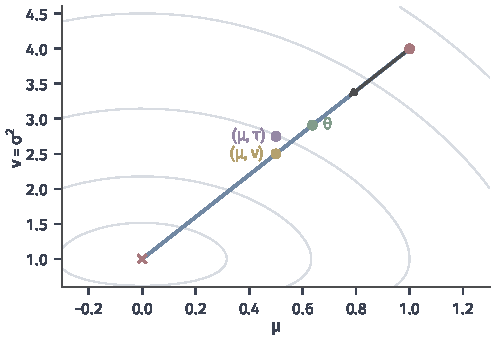
\includegraphics[width=84mm]{figures/07-probability/07-distribution-optimization/matplotlib/igeo-finite-steps/figure.pdf}
  \caption{从$\mathcal{N}(1,4)$（红点）出发、步长$\alpha=\frac18$的一步自然梯度更新，画在$(\mu,v)$平面上，目标为$\mathcal{N}(0,1)$（红叉）。蓝线是自然梯度流，深灰箭头是三套坐标共同的切方向。黄、绿、紫三点分别是在$(\mu,v)$、自然参数$\theta$、$(\mu,\tau)$坐标中直接相加得到的新分布。浅灰线为$L$的等值线。}
  \label{fig:igeo-finite-steps}
\end{BookInlineFigure}

图~\ref{fig:igeo-finite-steps}中，$(\mu,v)$与自然参数两步恰好落在流的直线上，只是走得远近不同；$(\mu,\tau)$一步偏离了这条线。三者一阶相同，二阶以上的差别来自“在坐标中走直线”这一规则本身。若要求有限步也与坐标无关，需要规定从切向量回到参数空间的方式，例如沿Fisher度量的测地线走，或者采用某种满足一阶条件的回缩，这正是流形上的迭代要处理的问题。实际中，这种依赖性通过选择合适的坐标和足够小的步长来控制，并由目标值与参数可行性来检查。
